\documentclass[a4paper,12pt]{report}

\usepackage[utf8x]{inputenc}
\usepackage[T2A]{fontenc}
\usepackage[english, russian]{babel}

% Опционно, требует  apt-get install scalable-cyrfonts.*
% и удаления одной строчки в cyrtimes.sty
% Сточку не удалять!
% \usepackage{cyrtimes}

% Картнки и tikz
\usepackage{graphicx}
\usepackage{tikz}
\usetikzlibrary{snakes,arrows,shapes}


% Увы, поля придётся уменьшить из-за листингов.
\topmargin -1cm
\oddsidemargin -0.5cm
\evensidemargin -0.5cm
\textwidth 17cm
\textheight 24cm

\sloppy



% Оглавление в PDF
\usepackage[
bookmarks=true,
colorlinks=true, linkcolor=black, anchorcolor=black, citecolor=black, menucolor=black,filecolor=black, urlcolor=black,
unicode=true
]{hyperref}

% Для исходного кода в тексте
% \newcommand{\Code}[1]{\texttt{#1}}

% Некоторая русификация.
% \usepackage{misccorr} % Oh shi^W^W, оно не работает с report.
\usepackage{indentfirst}
\renewcommand{\labelitemi}{\normalfont\bfseries{--}}

% На дворе XXI век, но пакет listings всё ещё не пашет с русскими комментариями!

% Пакет listings для простой вставки исходников
% \usepackage{listings}
% Параметры оформления
% \lstset{
% showspaces=false,
% showtabs=false,
% frame=single,
% tabsize=4,
% basicstyle=\ttfamily,
% identifierstyle=\ttfamily,
% commentstyle=\itshape,
% stringstyle=\ttfamily,
% keywordstyle=\ttfamily,
% breaklines=true
% }
% Русский в комментариях.
% \lstset{escapebegin=\begin{cyr},escapeend=\end{cyr}}



% А это взято из файла, сгенерённого doxygen
\usepackage{calc}
\usepackage{array}
\newenvironment{Code}
{\footnotesize}
{\normalsize}
\newcommand{\doxyref}[3]{\textbf{#1} (\textnormal{#2}\,\pageref{#3})}
\newenvironment{DocInclude}
{\footnotesize}
{\normalsize}
\newenvironment{VerbInclude}
{\footnotesize}
{\normalsize}
\newenvironment{Image}
{\begin{figure}[H]}
{\end{figure}}
\newenvironment{ImageNoCaption}{}{}
\newenvironment{CompactList}
{\begin{list}{}{
  \setlength{\leftmargin}{0.5cm}
  \setlength{\itemsep}{0pt}
  \setlength{\parsep}{0pt}
  \setlength{\topsep}{0pt}
  \renewcommand{\makelabel}{\hfill}}}
{\end{list}}
\newenvironment{CompactItemize}
{
  \begin{itemize}
  \setlength{\itemsep}{-3pt}
  \setlength{\parsep}{0pt}
  \setlength{\topsep}{0pt}
  \setlength{\partopsep}{0pt}
}
{\end{itemize}}
\newcommand{\PBS}[1]{\let\temp=\\#1\let\\=\temp}
\newlength{\tmplength}
\newenvironment{TabularC}[1]
{
\setlength{\tmplength}
     {\linewidth/(#1)-\tabcolsep*2-\arrayrulewidth*(#1+1)/(#1)}
      \par\begin{tabular*}{\linewidth}
             {*{#1}{|>{\PBS\raggedright\hspace{0pt}}p{\the\tmplength}}|}
}
{\end{tabular*}\par}
\newcommand{\entrylabel}[1]{
   {\parbox[b]{\labelwidth-4pt}{\makebox[0pt][l]{\textbf{#1}}\vspace{1.5\baselineskip}}}}
\newenvironment{Desc}
{\begin{list}{}
  {
    \settowidth{\labelwidth}{40pt}
    \setlength{\leftmargin}{\labelwidth}
    \setlength{\parsep}{0pt}
    \setlength{\itemsep}{-4pt}
    \renewcommand{\makelabel}{\entrylabel}
  }
}
{\end{list}}
\newenvironment{Indent}
  {\begin{list}{}{\setlength{\leftmargin}{0.5cm}}
      \item[]\ignorespaces}
  {\unskip\end{list}}



\title{Отчёт по курсовому проекту }
\author{(Пучнина Анастасия Ивановна, Козлова Юлия Алексеевна)}

\begin{document}

\maketitle

\tableofcontents

\addcontentsline{toc}{chapter}{Введение}
\chapter*{Введение}

\section{Серверная часть SMTP агента}

\subsection{Задание. Вариант 10}

Используется вызов pselect и единственный рабочий поток. Журналирование в отдельном процессе. Нужно проверять обратную зону днс.

\subsection{Цель и задачи}

Цель:
    Разработать \textbf{SMTP-сервер} с использованием одного потока и метода pselect().

Задачи:
\begin{itemize}
    \item проанализировать архитектурное решение;
    \item разработать подход для обработки входящих соединений;
    \item разработать подход хранения входящих писем в maildir;
    \item проанализировать \textbf{SMTP}-протокол и разработать конечный автомат обработки SMTP-сообщений;
    \item реализовать программу для получения и сохранения писем по протоколу \textbf{SMTP}.
\end{itemize}

\section{Клиентская часть SMTP агента}

\subsection{Задание. Вариант 31}

Используется вызов select и единственный рабочий поток (или процесс). Журналирование в отдельном процессе. Пытаться отправлять все сообщения для одного MX за одну сессию.

.... % Юле сюда надо добавить свою часть

\chapter{Аналитический раздел}

\section*{Предметная область}

\subsection*{ER-диаграмма предметной области}

В результате проведенного исследования были выявлены следующие сущности предметной области:

\begin{enumerate}
    \item Отправитель.
    \item Получатель.
    \item Пользователь.
    \item Электронное письмо.
    \item Файл письма.
    \item Каталог Maildir.
\end{enumerate}

Зависимость между сущностями предметной области может быть описана ER-диаграммой (~\ref{fig:er_diagram} ). Диаграмма выполнена в соответствии с нотацией UML.
\begin{figure}
    \centering
    \includegraphics[width=\textwidth]{../images/er_diagram.png}
    \caption{ER-диаграмма предметной области}
    \label{fig:er_diagram}
\end{figure}


\section*{Достоинства и недостатки реализуемой архитектуры}

\subsection*{Серверная часть SMTP агента}

Согласно условию задачи, в работе сервера предлагается использовать один поток выполнения и один отдельный поток
журналирования.

Достоинства данного варианта реализации:
\begin{itemize}
    \item простота реализации, отсутствует необходимость реализации разделяемой памяти и взаимодействия между процессами или потоками;
    \item отсутствие времени на переключение контекстов;
    \item благодаря неблокирующему вводу/выводу, сервер может обслуживать множество клиентов с достаточно высокой производительностью, при условии, что обработка занимает мало времени;
    \item логирование в отдельном процессе позволяет не блокироваться на операциях ввода/вывода при записи в файл или в терминал;
\end{itemize}

Недостатки данной архитектуры:
\begin{itemize}
    \item низкая производительность при длительной обработке клиентских команд;
    \item низкая отказоустойчивость (использование одного потока является менее надежным при возникновении фатальных ошибок в приложении, чем при наличии нескольих взаимозаменяемых потоков,);
    \item сложность масштабирования и использования всех аппаратных ресурсов системы.
\end{itemize}

Недостатки программной реализации с одним потоком выполнения и мультиплексированием можно уменьшить с  помощью
создания нескольких (пула) потоков с неблокирующим вводом/выводом и распределения нагрузки между ними.

\subsection*{Клиентская часть SMTP агента}

.... % Юле сюда надо добавить свою часть

\chapter{Конструкторский раздел}

\section{Конечный автомат состояний сервера}

На рис.~\ref{fig:server_fsm} представлен сгенерированный с использованием \textit{fsm2dot} скрипта из \textit{autogen}
файла конфигурации конечного автомата \textit{serverfsm.def} и \textit{dot}.

Данный рисунок не отображает переходы между состояниями при использовании именнованных обработчиков,
поэтому, для корректного отображения конечного автомата, был создан специальный файл конфигурации
\textit{serverfsm_report.def} без использования в \textit{autogen} параметров \textit{ttype} в переходах автомата.
Построенный таким образом граф состояний представлен на рис.~\ref{fig:server_fsm_report}.

\begin{figure}
    \centering
    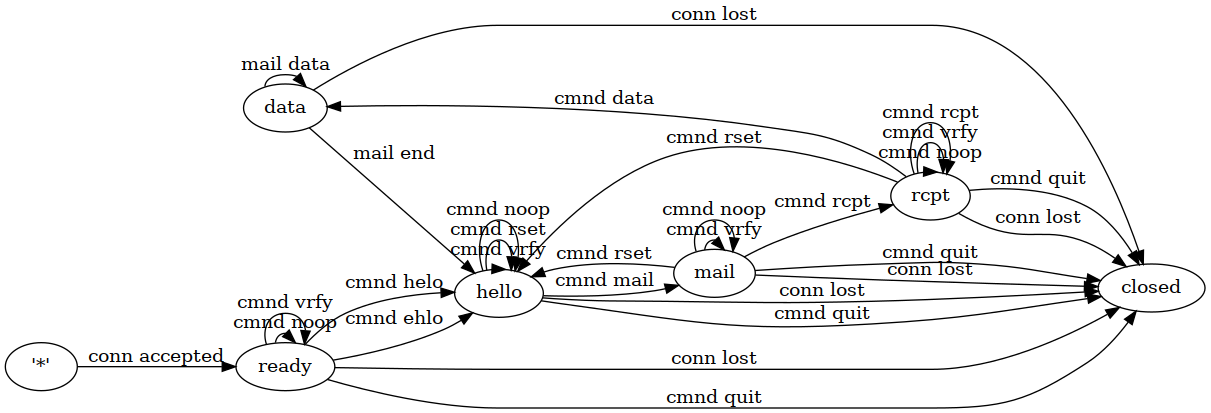
\includegraphics[width=\textwidth]{../images/serverfsm.png}
    \caption{Построенный граф конечного автомата SMTP сервера с использованием именнованных обработчиков}
    \label{fig:serverfsm_def}
\end{figure}

\begin{figure}
    \centering
    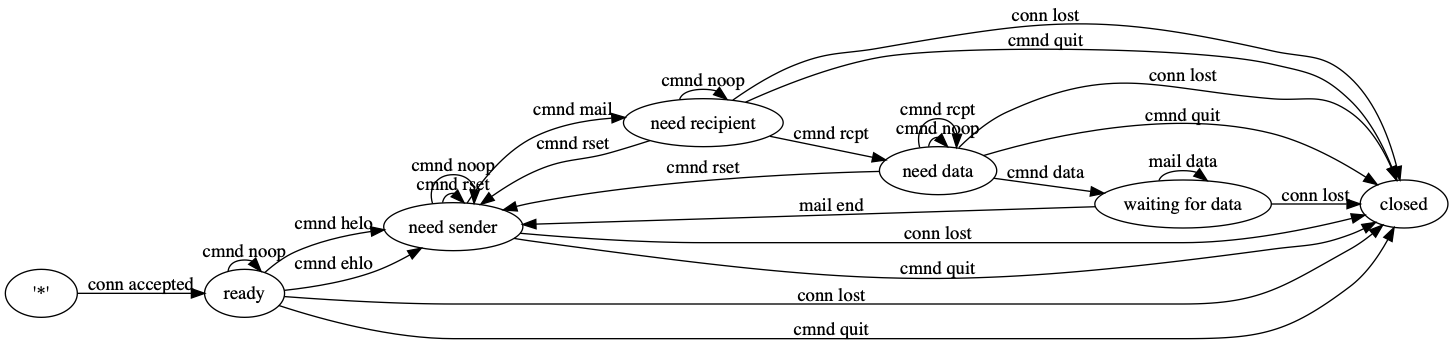
\includegraphics[width=\textwidth]{../images/serverfsm_report.png}
    \caption{Граф состояний конечного автомата SMTP сервера}
    \label{fig:serverfsm_report_def}
\end{figure}


\section{Синтаксис команд протокола}
Ниже приведен формат команд сообщений протокола в виде регулярных выражений:

Общие регулярные выражения:
\begin{description}
\item[Перевод строки]
\texttt{\textbackslash{}\textbackslash{}r\textbackslash{}\textbackslash{}n}
\item[Пробелы]
\texttt{\textbackslash{}s*}
\item[Доменное имя]
\texttt{<?<domain>.+>}
\item[Электронный адрес или пустые скобки]
\texttt{<?<address>.+@.+>|<>}
\item[Электронный адрес]
\texttt{<?<address>.+@.+>}
\end{description}

Регулярные выражения SMTP команд:
\begin{description}
    \item[NOOP]
    \texttt{\^{}NOOP}
    \item[HELO]
    \texttt{[Hh][Ee][Ll][Oo]\textbackslash{}\textbackslash{}s*(?<domain>.+)\textbackslash{}\textbackslash{}r\textbackslash{}\textbackslash{}n}
    \item[EHLO]
    \texttt{\^{}EHLO:}
    \item[MAIL]
    \texttt{\^{}MAIL FROM:}
    \item[RCPT]
    \texttt{[Rr][Cc][Pp][Tt] [Tt][Oo]:\textbackslash{}\textbackslash{}s*<(?<address>.+@.+)>\textbackslash{}\textbackslash{}r\textbackslash{}\textbackslash{}n}
    \item[VRFY]
    \texttt{\^{}VRFY:}
    \item[DATA]
    \texttt{\^{}DATA}
    \item[RSET]
    \texttt{[Rr][Ss][Ee][Tt]\textbackslash{}\textbackslash{}r\textbackslash{}\textbackslash{}n}
    \item[QUIT]
    \texttt{\^{}QUIT}
\end{description}

Регулярные выражения содержимого письма:
\begin{description}
    \item[Данные письма]
    \texttt{[\textbackslash{}x00-\textbackslash{}x7F]+}
    \item[Окончание данных письма]
    \texttt{\^{}\textbackslash{}.}
\end{description}

\section{Синтаксис команд протокола}
На рис.~\ref{fig:uml_server_ph} и на рис.~\ref{fig:uml_server_log} представлены физическая и логическая
диаграммы представления данных в системе соответственно.

\begin{figure}
    \centering
    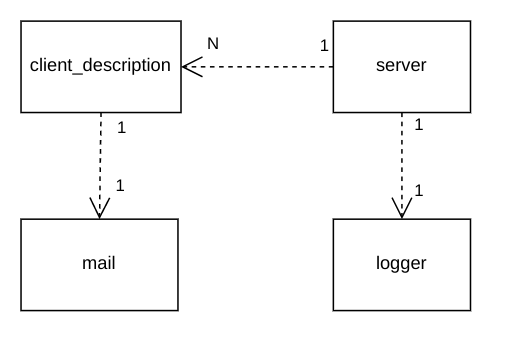
\includegraphics[width=\textwidth]{../images/uml_server_ph.png}
    \caption{Физическая диаграмма представления данных в серверной части системы}
    \label{fig:uml_server_ph}
\end{figure}

\begin{figure}
    \centering
    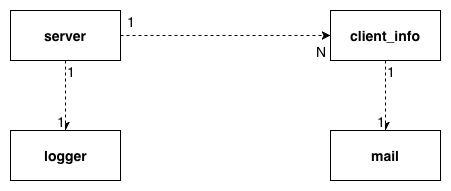
\includegraphics[width=\textwidth]{../images/uml_server_log.png}
    \caption{Логическая диаграмма представления данных в серверной части системы}
    \label{fig:uml_server_log}
\end{figure}


Конфигурация \textit{serveropts.def}, используемая для автоматической генерации исходного кода обработки
входных флагов приложенияс помощью \textit{autogen}.:

\lstset{language=C}
\lstinputlisting{../../source/server/autogen/serveropts.def}

\chapter{Технологический раздел}

\section{Сборка программы}

Сборка SMTP агента состоит из трех \textit{Makefile} системы сборки \textit{make}:

\begin{itemize}
    \item сборка клиента,
    \item сборка сервера,
    \item сборка отчета.
\end{itemize}

\subsection{Сборка серверной части SMTP агента}

Сборка SMTP сервера состоит из следующих целей:

\begin{enumerate}
    \item сборка сервера;
    \item сборка тестового клиента;
    \item генерация исходных кодов конечного автомата и опций с помощью \textit{autogen};
    \item сборка сервера и тестового клиента;
    \item запуск системного тестирования.
\end{enumerate}

Сборка программы осуществляется с помощью следующей команды:
\begin{verbatim}
    make autogen_all && make all
\end{verbatim}


\addcontentsline{toc}{chapter}{Выводы}

\chapter*{Выводы}

\section{Серверная часть SMTP агента}

В результате выполнения курсового проекта была достугнута поставленная цель, а именно разработан
\textbf{SMTP-сервер} с использованием одного потока и метода pselect(), осуществляющее прием и сохранение писем
для дальнейшей поставки их пользователям.

Во время выполнения работы были выполнены следующие задачи:
\begin{itemize}
    \item проанализировано архитектурное решение, данное по условиям задачи, определены его преимущества и недостатки;
    \item разработан и реализован подход для обработки входящих соединений на основе метода pselect();
    \item разработан и реализовано хранение входящих писем в каталоге maildir;
    \item проанализирован протокол \textbf{SMTP} и реализован конечный автомат обработки входящих SMTP-сообщений;
\end{itemize}

А также получены и закреплены следующие навыки:
\begin{itemize}
    \item проектирование и реализация сетевого протокола SMTP;
    \item реализация серверного приложения с несколькими процессами на языке программирования Си;
    \item создание сценариев сборки программного обеспечения;
    \item использование latex и сценариев сборки для автогенерации расчетно-пояснительной записки.
\end{itemize}

В ходе работы не были реализованы следующие пункты, планируемые к разработке в дальнейшем:
\begin{itemize}
    \item проверка обратной зоны DNS;
    \item генерация документации и графов функци с помощью утилит;
    \item использование внешних конфигурационных файлов;
    \item модульное тестирование;
\end{itemize}


\end{document}
